
\documentclass[10pt]{article}

% amsmath package, useful for mathematical formulas
\usepackage{amsmath}
% amssymb package, useful for mathematical symbols
\usepackage{amssymb}

% graphicx package, useful for including eps and pdf graphics
% include graphics with the command \includegraphics
\usepackage{graphicx}
\usepackage{wrapfig}
% cite package, to clean up citations in the main text. Do not remove.
\usepackage{cite}

\usepackage{color} 

% Use doublespacing - comment out for single spacing
%\usepackage{setspace} 
%\doublespacing


% Text layout
\topmargin 0.0cm
\oddsidemargin 0.5cm
\evensidemargin 0.5cm
\textwidth 16cm 
\textheight 21cm

% Bold the 'Figure #' in the caption and separate it with a period
% Captions will be left justified
\usepackage[labelfont=bf,labelsep=period,justification=raggedright]{caption}

% Use the PLoS provided bibtex style
\bibliographystyle{plos2009}

% Remove brackets from numbering in List of References
\makeatletter
\renewcommand{\@biblabel}[1]{\quad#1.}
\makeatother


% Leave date blank
\date{}

\pagestyle{myheadings}
%% ** EDIT HERE **


%% ** EDIT HERE **
%% PLEASE INCLUDE ALL MACROS BELOW

%% END MACROS SECTION

\begin{document}

% Title must be 150 characters or less
\begin{flushleft}
{\Large
\textbf{Committee report: May 2013}
}
% Insert Author names, affiliations and corresponding author email.
\\
Sara Steele, co-authors Daniel Tranchina and John Rinzel
\end{flushleft}

\section*{Introduction}
For some stimuli in the visual and auditory modalities with ambiguous grouping cues, there is a tendency for the likelihood of perceptual "splitting" to increase with time. For instance, with ambiguous moving plaids constructed from moving square wave gratings at intermediate speed and angle, observers have consistently reported first experiencing motion coherence, even when steady-state perception is biased towards transparent motion of the individual gratings \cite{Rubin2004}. Analogously, for ambiguous tone sequences in which observers report alternations between hearing grouped triplet patterns and split streams \cite{Noorden1975} (see Figure \ref{fig:percepts_timecourse}), there can be an initial period of buildup over which the probability of stream segregation increases. 

\newpage
\begin{figure}[scale = 0.6]
	\centering
	\includegraphics[scale=0.35]{../aba_stimulus-percepts}
	
\includegraphics[scale=0.45]{../percepts_timecourse}
	\caption{}
	\label{fig:percepts_timecourse}
\end{figure}

Buildup is thought to reflect the accumulation of evidence by the sensory system to support the representation of multiple objects in a complex scene \cite{Bregman}, or alternatively the accumulation of multi-second habituation of the neurons processing acoustic inputs \cite{Micheyl2005}, \cite{Pressnitzer2008}. However, we show that this need not be the rule for the neural hardware underlying the subjectively sudden, stochastic switches between perceptual states; alternatively, the apparently gradual increase in probability of a split percept over time could be the averaging over many trials of a process that switches suddenly, but randomly, from a known starting state, and then alternates.

Indeed, the process of constructing buildup curves reflects the averaging over many trials of binary timecourses (see Figure \ref{fig:TrialAvg}). We believe that the observation that the starting state is fixed is sufficient to account for transient increase in probability of split percepts, but that buildup is primarily a consequence of stochastic alternations between two states.

\begin{figure}
	\centering
	\includegraphics[scale=0.35]{../percepts_timecourse_binary}
	\includegraphics[scale=0.5]{../TrialAvg}
	\caption{}
	\label{fig:TrialAvg}
\end{figure}

We tested whether perceptual bistability models were capable of producing realistic buildup curves if the starting state was fixed, and under which dynamical regimes.
\cite{Shpiro2009}

\begin{figure}
	\centering
	\includegraphics[scale=0.5]{../lit_buildup}
	\caption{Buildup curves from \cite{Micheyl2005} (top) and \cite{Deike2012} (bottom). In Deike, buildup curves are modified by normalizing the average response at a particular timepoint by whether a response has been collected at that time point (rather than default value before a response has been made zero, assuming grouped starting percept)}
	\label{fig:lit_buildup}
\end{figure}

\section*{Methods}
\subsection*{Competition model simulations}
Competition model simulations followed the procedures reported previously in \cite{Shpiro2009} for population firing rate model with spike frequency adaptation. Specifically,

\begin{equation*}
	\begin{cases}
	\dot{u}_1 & = -u_1 +  f(-\beta u_2 - \gamma a_1 + I_1 + n_1) \\
	\tau_a \dot{a}_1 & = -a_1 + u_1\\
	\dot{n}_1 & = \frac{-n_1}{\tau_n} + \sigma \sqrt{\frac{2}{\tau_n}} \eta(t)\\
	\dot{u}_2 & = -u_2 +  f(-\beta u_1 - \gamma a_2 + I_2 + n_2) \\
	\tau_a \dot{a}_2 & = -a_2 + u_2\\
	\dot{n}_2 & = \frac{-n_2}{\tau_n } + \sigma \sqrt{\frac{2}{\tau_n}} \eta(t)
	
	\end{cases}
\end{equation*}

The variable $u_1$ corresponding to the short-time averaged firing rate of the population representing the ``grouped" perceptual state, and $u_2$ the firing rate of the population representing the ``split" perceptual state. The variables $a_1$ and $a_2$ represent the spike-frequency adaptation. Parameter $\gamma$ controls the strength of the adaptation, and $\beta$ controls the strength of suppression from the competing population. $I_1$ and $I_2$ are the external inputs driving the two populations, and $n_1$ and $n_2$ are independent Ornstein-Uhlenback noise generators with mean zero and variance $\sigma$, and a timescale of $\tau_n$. 
The input-output function used was a sigmoid, with $f (x) = 1/(1 + exp(−(x − \theta )/ k))$. 

The simulation was carried out on a characteristic neuronal timescale, with one unit of time corresponding to 10 msec. The following parameter values are used: $k = 0.1, \theta = 0, \beta = 1$. Time constants given in simulation time units were $\tau_a = 200, \tau_n = 10$. The values of the external inputs to the populations $I_1$ and $I_2$, the adaptation gain $\gamma$ and the noise strength $\sigma$ were varied as specified in the text, with the value of $\sigma$ scaled in relation to the integration time step by $1/\sqrt{dt}$ to keep specified variance per unit time. Simulations were implemented in MATLAB using forward Euler integration with a time step of 0.1 (1 msec real time).

For each combination of parameter values, we simulated 500 trials of length 10 s with initial conditions $u_2(0), a_1(0), a_2(0), n_1(0), n_2(0) = 0$ and $u_1(0) = 0.5$; thus, at the beginning of each simulated trial, the first population to become dominant was always that corresonding to the first percept. With the resulting population firing rate timecourses, we obtained dominance durations by finding time points of the zero crossings of the differences of the firing rates. Using the samples of dominance durations obtained for each population (over 1000 durations for each population with each parameter set), we fitted gamma densities using maximum likelihood estimation. Simulated experimental buildup curves were constructed by averaging across trials the binary timecourse $u_2 > u_1$. 

\subsection*{Derivation for alternating renewal process}
The solution to the alternating renewal process was implemented by solving a set of stochastic differential equations describing the rate of change in probability per unit time for each of the two states of a dichotomous random variable $z(t) = {0 , 1} $, as follows:

\begin{equation}
\frac{\partial f_0}{\partial t} \big(s,t\big) = -\frac{\partial}{\partial s}\big(1 * f_0(s,t)\big) - h_{T_0}(s) f_0(s,t)
\end{equation}

\begin{equation}
\frac{\partial f_1}{\partial t} \big(s,t\big) = -\frac{\partial}{\partial s} \big(1 * f_1(s,t)\big) - h_{T_1}(s) f_1(s,t)
\end{equation}

where $s(t)$ is the random elapsed time since entering state $i$ and $h_{T_i}(s)$ is the hazard function, the probability of exiting the current state in the interval $(t, t+dt)$. $h_{T_i}(s) = \dfrac{f_{T_i}}{\hat{F}_{T_i}}$, the ratio of the density function of durations $T_i$ for state i and its complementary cumulative distribution function.

The value of s is reset to 0 whenever an alternation between states occurs. The initial
probability source at s = 0 is determined by the probability of switches out of the previous state, leading to the following boundary conditions:

\begin{equation}
f_0(0,t) = \int_0^\infty h_{T_1}(s) f_1(s,t) ds
\end{equation}

\begin{equation}
f_1(0,t) = \int_0^\infty h_{T_0}(s) f_0(s,t) ds
\end{equation}

We used the following initial conditions, first solving for the case of beginning in state 1:

\begin{equation}
f_1(s,t=0) = \delta(s); f_0(s,t=0) = 0
\end{equation} 

Using these conditions yields the following solution:

\begin{equation}
f_{1}(t|z(0)=1) = \tilde{F}_{T_1}(t) + \frac{1}{2\pi} \int_{-\infty}^\infty dw \frac{1}{i\omega} \left[ \hat{\tilde{F}}_{T_1}(\omega) \hat{f}_{T_0}(\omega)\hat{f}_{T_1}(\omega) \frac{i\omega}{1 - \hat{f}_{T_0}(\omega)\hat{f}_{T_1}(\omega)} \right] e^{i \omega t}
\end{equation}
where $\hat{f}(x)$ is the Fourier transform of $f(x)$

To find the probability $f_1(t|z(0)=0)$, we time shift the above expression by the durations of the initial state, $T_0^0$, whose density function is $f_{T_0^0}(t)$. This amounts to a convolution of the density for initial durations (and first switch times) with the previous solution:

\begin{equation}
f_1(t|z(0)=0) = \int_0^t f_{T_0^0}(s) f_{1}([t-s]|z(0)=1) ds
\end{equation}

Thus the solution can be given in the Fourier domain as:
\begin{equation}
\hat{f}_{1|0}(\omega) = \hat{f}_{T_0^0}(\omega) \hat{p}_{1|1} (\omega)
\end{equation}

Using the simplifying assumption that ${f}_{T_0^0}(t) = {f}_{T_0}(t)$, that is, that the initial percept duration is from the same density function as all other $T_0$, we find:
 
\begin{equation}
\hat{f}_{1|0}(\omega) = \hat{\tilde{F}}_{T_1}(\omega)
\left( \hat{f}_{T_0} + \frac{\hat{f}_{T_0}^2(\omega)\hat{f}_{T_1}(\omega)}{1-\hat{f}_{T_0}(\omega)\hat{f}_{T_1}(\omega)}\right)
\end{equation}
At $\omega = 0, \hat{f}(\omega) = \mu(T_1) / (\mu(T_1) + mu(T_0)$. From here, the expression in the time domain is obtained by taking the inverse Fourier transform and finding the integral from 0 to t.  

\section*{Results}
 
\subsection*{Alternating renewal process provides robust fits using MLE gamma parameters to predict buildup, but not vice versa}
Using the four parameter implementation described above, in which starting duration assumed to be from same distribution as other grouped percept durations, we obtain strong predictions for the buildup function $(R^2 > .90)$ (see Figure \ref{fig:mono_vs_periodic}), even when adaptation is stronger and percept-to-percept correlations exist. This is remarkable because the assumptions of the alternating renewal process is that duration distributions are independent. However, the ability of the model to find strong fits under violations of its assumptions belie a nonspecific parameter space; the best-fitting least squares parameters for the buildup function poorly predict the underlying gamma density parameters (see Figure \ref{fig:gam_to_BUF}), and the buildup curve as currently formulated does not constrain well the distributions that produce it. Alternative formulations may do better.

\begin{figure}[scale = 0.8]
   \begin{center}
   
   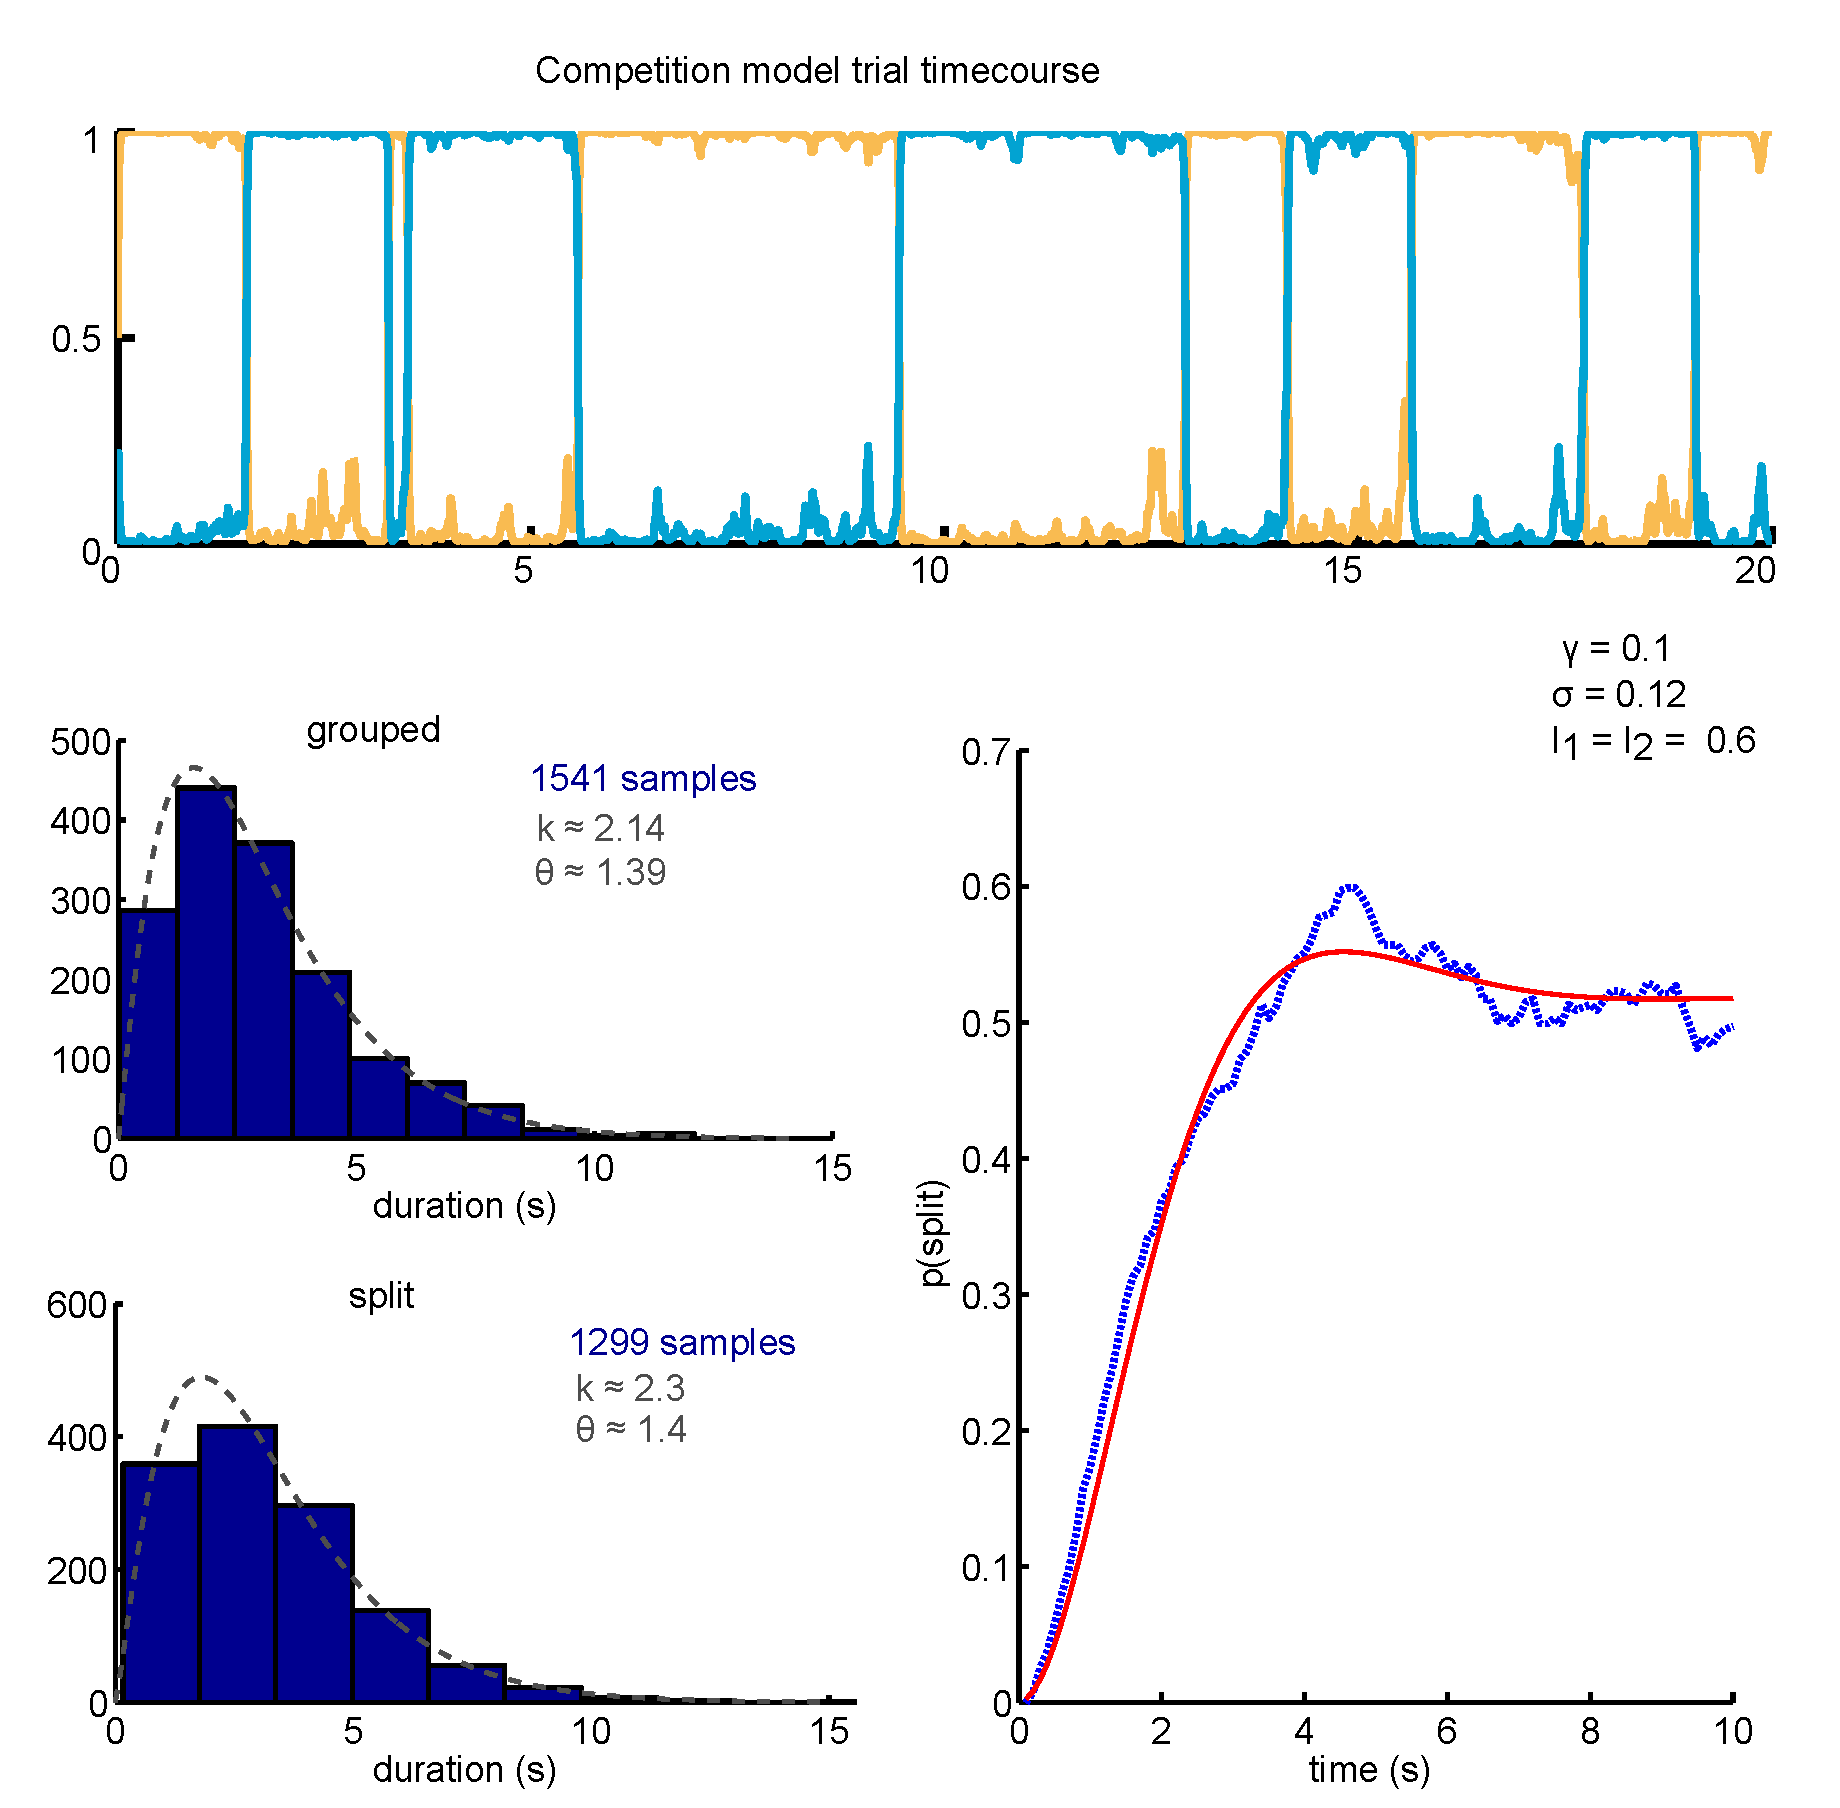
\includegraphics[scale=0.33]{BUFs_hists_lowadapt}
   
   \includegraphics[scale=.33]{hi_adapt_low_noise_equal_inputBUFshists}      
   \caption{Buildup functions for low-adaptation and high-adaptation, low noise parameter regimes.}
   	\label{fig:mono_vs_periodic}
   \end{center}
\end{figure}


\begin{figure}[scale=0.5]
   \begin{center}
   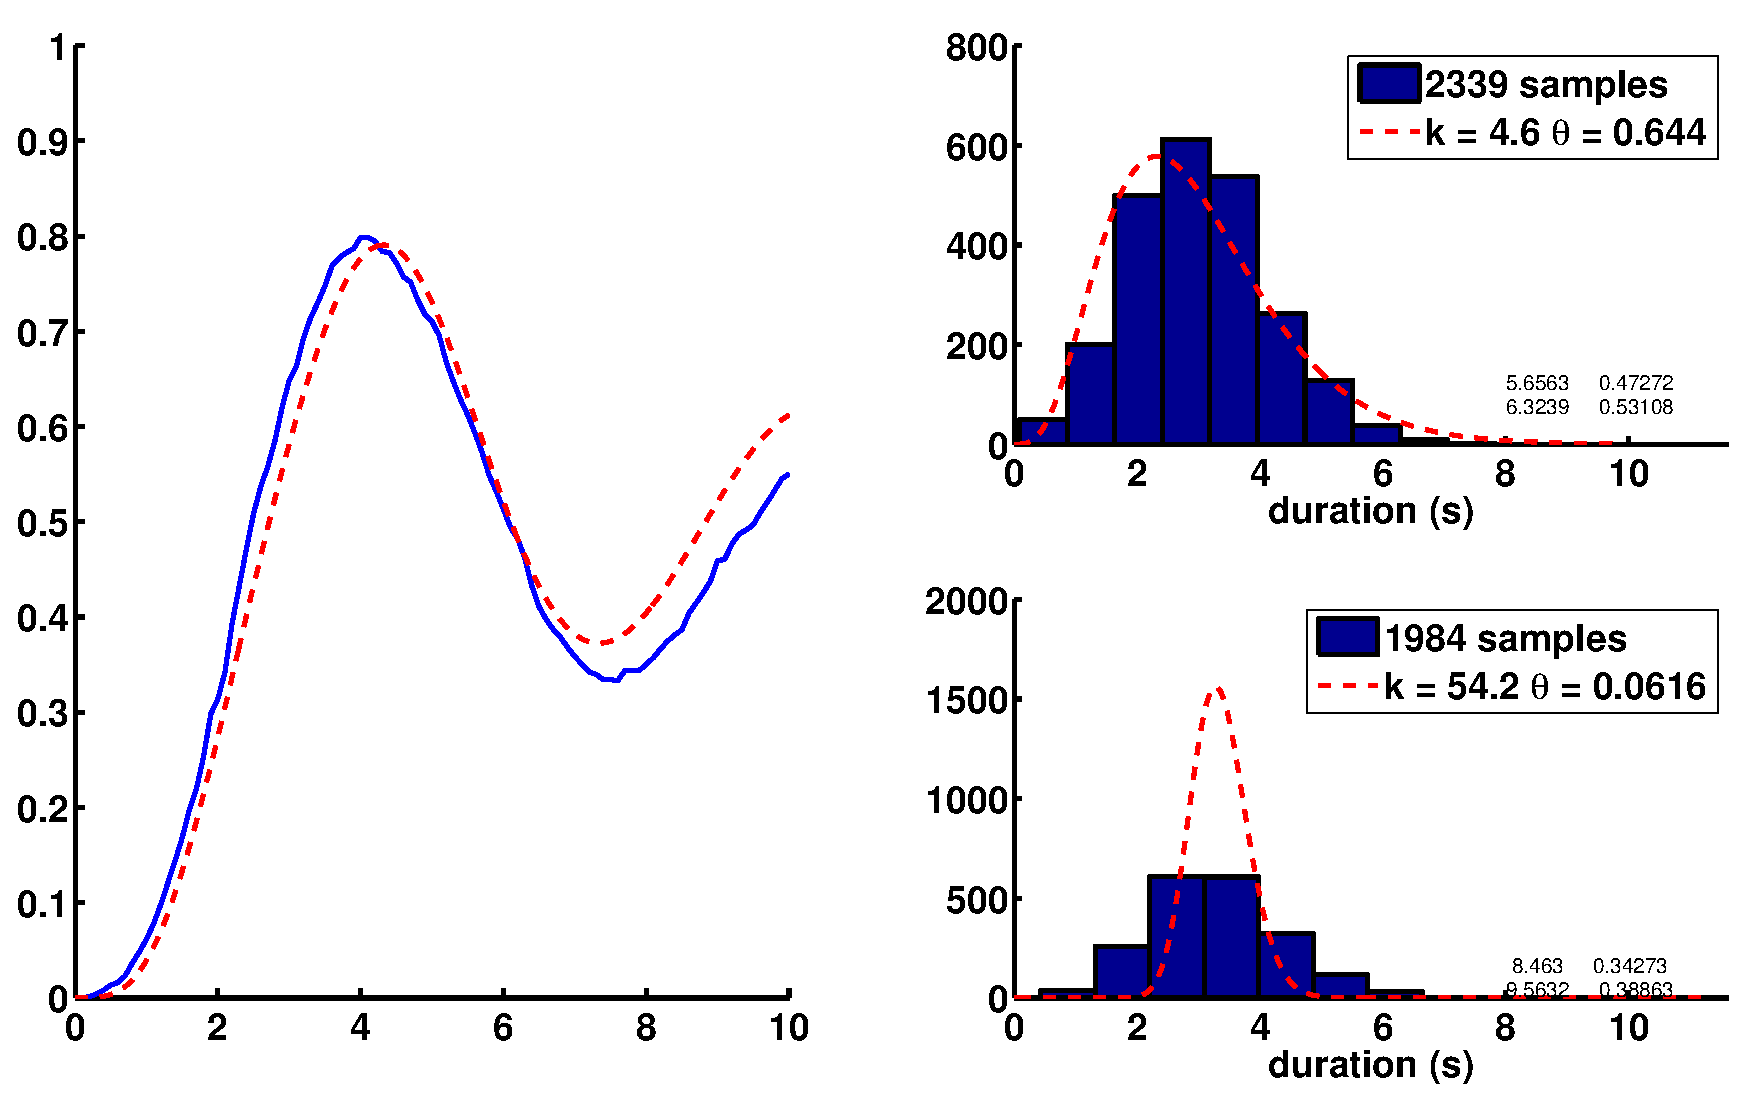
\includegraphics[scale=0.33]{../reverse_fit_lownoise_hiadapt}   
   \caption{}
   	\label{fig:gam_to_BUF}
   \end{center}
\end{figure}
%


\subsection*{Buildup curves look most realistic for noise-driven, not adaptation driven, alternation regimes}
See Figure \ref{fig:mono_vs_periodic}. Noise driven switching is necessary for buildup functions that look like those presented in the literature; however, in principle the apparent monotonically increasing likelihood of split percepts over time could also be accomplished by averaging together the timecourses of multiple oscillators with different periods. However, there have been no reports whatsoever of oscillatory buildup functions.



\begin{figure}[scale = 0.4]
   \begin{center}
   	\includegraphics[scale = 0.5]{../clocky_switches} % requires the graphicx package
   \caption{When switches are driven by adaptation, the system behaves as a noisy oscillator around a fixed period. Because of the "clockiness" of the timecourses, the oscillations appear in the average.}
   	\label{fig:example}
   \end{center}
\end{figure}




\subsection*{Buildup occurs faster for less ambiguous stimuli}

The time it takes to achieve the steady state fractional dominance ratio should depend on both how far the original fractional dominance ratio from the steady state as well as the strength of the biasing input in favor of either of the two states. In \ref{fig:ambiguous_vs_biased} we see that the strength of the biasing input is much more important to defining the overall timescale of buildup than the distance between starting and steady states. This effect is in contrast to the effect on mean durations; mean durations for grouped percepts in the ambiguous case was 8.07 s, and for split 7.57 (grand mean =  7.8) whereas for the biased case, the average grouped duration was 1.29 s, the averaged split duration was 18.213, and the grand mean was 9.75. So while switches occurred more frequently in the ambiguous case, the time to half-maximum was also longer.

\begin{figure}[scale=0.5]
   \begin{center}
   
   \includegraphics[scale=0.33]{../ambiguous_vs_biased}
   
   \caption{When stimulus is very ambiguous, leading to steady state equal fractional dominance durations, buildup is slow-- left, half-maximum is achieved after about 5 s. However when the stimulus is strongly biased, the steady state is achieved in much shorter time (~2s), even when this is further from the starting state.}
   	\label{fig:ambiguous_vs_biased}
   \end{center}
\end{figure}
%




\section*{Future Directions}
I am writing up the present results for publication in a computational journal, eg Frontiers of Computational Neuroscience.

The present method for producing simulated empirical buildup functions has some issues-- \cite{Hupe2012} among others show that the first percept is typically longer than subsequent grouped percepts. However, in my simulations the first percept winds up being shorter (see Figure \ref{fig:first_vs_other}). I believe this is because I force the first percept by setting the initial condition on population activity, thus that population accrues adaptation faster than if it were starting from zero activity. I believe I can fix this by setting the initial conditions on adaptation of the non-dominant-start population-- however it would be more interesting to find a stimulus-driven method of fixing the starting percept.

Mapping the objective function for least squares estimates of the four-parameter alternating renewal process buildup curve will help us understand why these fits do not constrain the duration probability densities. Furthermore, a more sophisticated implementation of the alternating renewal process, in which we include the different first-percept distribution (six parameter model, find first percept parameters first and use LSE to find the remaining four to predict dynamics over long trials from the buildup function) may yield stronger predictions.

\begin{figure}[scale=0.5]
   \begin{center}
   
   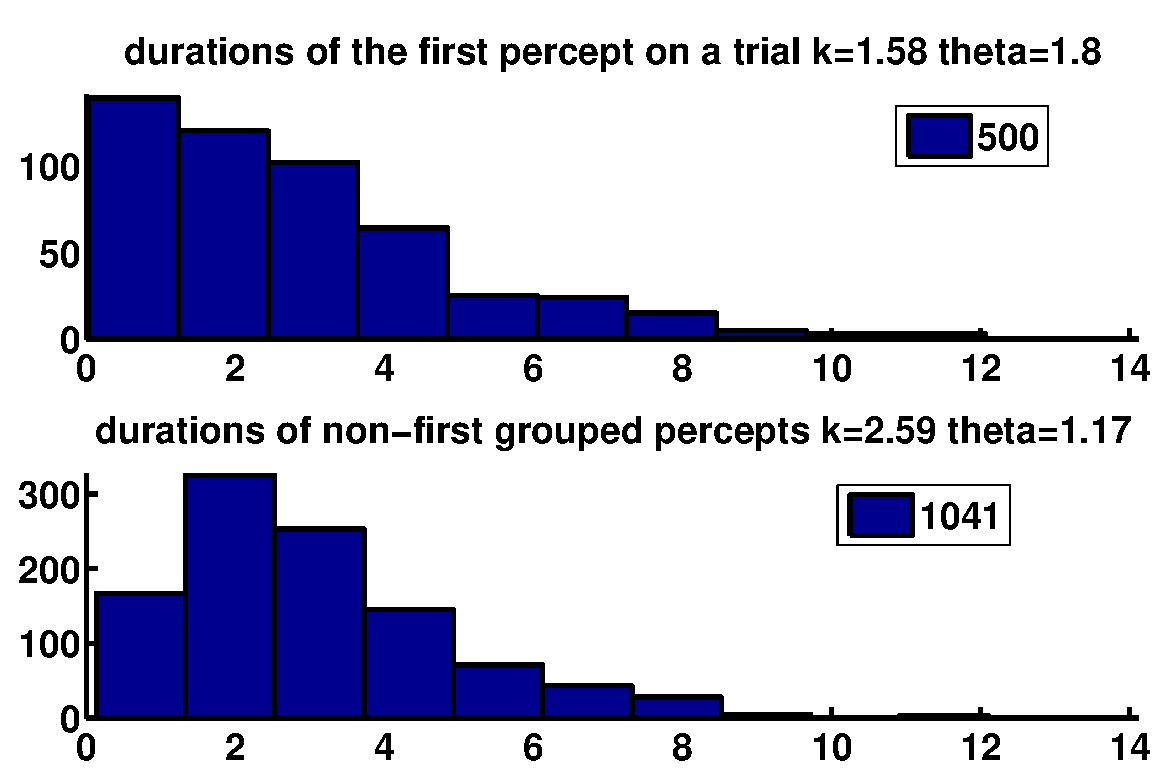
\includegraphics[scale=0.33]{../first_vs_other_hists}
   
   \caption{}
   	\label{fig:first_vs_other}
   \end{center}
\end{figure}



A number of stimulus-specific effects have been described, as well as prior-state effects. For instance, it takes many seconds of silence for buildup to re-set, unless the stimulus is restarted in a different frequency band (Jon Sussman). In addition, prior exposure to larger frequency differences biases subsequent perception of a more ambiguous stimulus towards "grouped" (repulsive), and vice versa \cite{Snyder2009}. I would like to try to build models that capture these effects by including more features of the peripheral auditory system and perhaps a short term memory component.


\section*{References}
% The bibtex filename
\bibliography{/Users/steeles/Documents/library}


\end{document}